

The goal of our fast path  is to forgo the overhead associated with two-phase transaction processing and communication with 
the TM to begin and commit transactions. This is particularly important for short transactions, where the begin and commit overhead is not amortized
across many operations.
We therefore focus on single-key transactions.

To this end, we introduce in Section~\ref{ssec:fast-api} a streamlined  \emph{fast path (FP)}
API that jointly executes multiple API calls of the original TPS, and 
%we refer to transactions that use this API as \emph{fast path (FP) transactions}. We 
define the semantics of FP transactions relative to regular ones.
% in Section~\ref{ssec:fast-semantics}.
We proceed, in Section~\ref{ssec:fast-algorithm}, to explain our general fast path algorithm 
\inred{for any system that follows the generic schema of  Algorithm~\ref{alg:schema} above}. 
Finally, in Section~\ref{ssec:fast-impl}, we describe our implementation of the fast path in \sys, and 
important practical optimizations we did in this context.
 

 \remove{
   with SI semantics in the
context of a system following the generic schema of  Algorithm~\ref{alg:schema} above. 
Our solution consists of three parts: First, in Section~\ref{ssec:region-clock}, we enhance the
underlying data store with support for per-region \emph{Local Version Clocks (LVCs)}. 
This aspect is already implemented in CockroachDB, which uses 
per-region Hybrid Logical Clocks~\cite{Kulkarni2014LogicalPC} in order to allow for distributed timestamp allocation. 
In the systems that maintain a GVC, (e.g.,~\cite{Percolator2010,tephra,OmidICDE2014,omid-blog}), our 
addition of  LVCs 
entails a minor modification to management of global timestamps (in the transaction manager or oracle). 
Second, in Section~\ref{ssec:lvc-access}
we extend the underlying data store's API to allow manipulating 
a region's LVC jointly with objects stored at that region. 
Finally, we add client-side support for the fast path API, as explained in Section~\ref{ssec:lc-client}.
}

\subsection{API and semantics}
\label{ssec:fast-api}

\paragraph{API.}
For brevity, we refer to the TPS's API calls  begin, read, write, and commit as \code{b, r, w}, and \code{c} respectively, and 
we combine them to allow fast processing.
The basic FP transactions are singletons, i.e., transactions that perform a single
read or write. These are supported by the APIs: 
\begin{description}
\item[brc(key)] -- begins an FP transaction, reads key within it, and commits.
%Recall that read-only transactions don't need to commit. 
\item[bwc(key,val)] -- begins an FP transaction,  writes val into a new version of key that exceeds all existing ones, and commits.
\end{description}

We further support a fast path transaction consisting of a read and a dependant write, via a pair of API calls:
\begin{description}
\item[br(key)] -- begins an FP transaction and  reads the latest version of key.
\item[wc(key,val)] -- 	validates that key has not been written since the last \code{br} call, writes val into a new version of key, and commits.
\end{description}

\remove{
A more elaborate example is a read-modify-write API: 
\begin{description}
\item[brwc(key,f)] -- begins an FP transaction,  reads the latest version of key, applies $f$ to it (on the server side), 
	writes the result into a new version of key that exceeds all existing ones, and commits.
\end{description}

To use the above API, the programmer has to encapsulate the transaction logic in a function for server-side processing. 
Alternatively, we allow FP transactions to unfold dynamically much like regular  transactions do.
A dynamic FP transaction may instead begin with a \code{br} call, perform client-side processing, and then call the following
function to update either the same or a different key: 

\begin{description}
\item[wc(key,val)] -- writes val into a new version of key that exceeds all existing ones, and commits.
\end{description}

Moreover, we do not restrict FP transactions to perform a single read -- any number of \code{r}'s may be called between the \code{br} 
and \code{wc}. The supported types of FP transactions are summarized in Table~\ref{table:fp-types}.
Note, however, that all calls must be directed at the same region, else the transaction is not local.
In case an FP transaction dynamically discovers that it needs to access additional regions, it is aborted and should be restarted as a regular transaction. 

\begin{table}[htb]
%\def\arraystretch{1.5}%  1 is the default, change whatever you need
\centerline{
\begin{tabular}{l  @{\hspace{2em}} l}
Call sequence & Transaction type\\
\hline
\code{br} & single read\\
\code{bwc} & single write\\
\code{br, r*} &  multi-read\\
\code{br, r*, wc} & multi-read, single write\\
\code{brwc} & server-side single-read-write\\
%\hline
\end{tabular}
}
\caption{Supported FP transaction types.}
\label{table:fp-types}
\end{table}

In principle, it would have been possible to also allow \code{w} calls in the span of an FP transaction, 
but in this case, it is not possible to forgo the two-phase execution. 
That is, the \code{w} calls would need to indicate write intents, and  to be atomically committed (or aborted) during the final \code{wc} 
(or \code{c}) call. 
Given the limited benefit and extra complexity of allowing many writes in FP transactions, we do not support this option in our solution.

}

\paragraph{Semantics.}
%\label{ssec:fast-semantics}

The semantics for ordering FP transactions relative to regular ones are
weaker than SI in that they do not guarantee real-time order over all regular
and FP transactions together. For example, an FP tranasction may return 
an older value than the latest one committed by a regular transaction. Similarly, a regular transaction overlapping
two FP ones may observe an update of the second and miss an update by the first,  as illustrated in Figure~\ref{fig:ltx-rt}.

\begin{figure}[h]
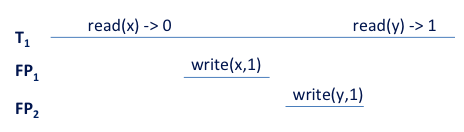
\includegraphics[width=\columnwidth]{figs/FP-semantics}
\caption{Possible violation of real-time order among fast path (FP) transactions. Regular transaction $T_1$
reads $x$ before it is updated by FP transaction $FP_1$ and reads $y$ after it is updated by FP transaction $FP_2$ even 
though $FP_2$ occurs after $FP_1$. 
%$T1$'s global version is $10$, and its skips the local version clocks of the regions holding $x$ and $y$ to $10$ when reading from them.
}
\label{fig:ltx-rt}
\end{figure}

The system still enforces a total order ${\cal T}$ on all committed transactions, so that
\begin{enumerate}
    \setlength{\itemsep}{0pt}
    \setlength{\parskip}{0pt}
    \setlength{\parsep}{2pt}  
\item
regular transactions (though not FP ones) are ordered in ${\cal T}$  according to their commit times;
\item
each regular transaction's read operations see a consistent snapshot of the database reflecting 
a prefix of  ${\cal T}$ that includes all transactions committed prior to
its start time plus any number of concurrent FP transactions; and 
\item
 a transaction commits only if none of the items it updates has been modified since that snapshot.
 \end{enumerate}

Note that  ${\cal T}$  preserves causality because 
only transactions that  access different data objects can be re-ordered.


\subsection{Generic fast path algorithm}
\label{ssec:fast-algorithm}



\begin{algorithm}[htb]
\begin{algorithmic}
\State local variable \code{ts$_r$} \Comment timestamp read by ongoing transaction
\Statex
\Procedure{brc}{key}
\State
return latest non-tentative version of key
\EndProcedure
\Statex
\Procedure{bumpVersion}{key, $ts_r$} 
\Statex \Comment performed by transactional read
\EndProcedure
\Statex
\Procedure{bwc}{key, value} 
\State  TODO
\EndProcedure
\Statex
\Procedure{br}{key} 
\State $\langle$ \code{ts$_r$}, value  $\rangle \leftarrow$ getWithTs(key)
\State  return value
\EndProcedure
\Procedure{wc}{key, value} 
\State TODO
\EndProcedure

\end{algorithmic}
\caption{Generic support for FP transactions.}
\label{alg:fp}
\end{algorithm}

The generic fast fast path algorithm is given in Algorithm~\ref{alg:fp}. 
%
Single-read transactions simply return the latest committed version of the requested key they encounter.  
They ignore tentative versions, which may lead to missing the latest commit, but is allowed by our semantics. 
FP reads can forgo the begin call since they do not need to obtain a snapshot time a priori. 
They can also forgo the commit call, since the consistency of their snapshot does not need to be validated.
 
Single-write transactions need to produce a new version that exceeds all committed ones.  
To this end, they need to be able to determine the latest committed version. Thus, 
in case a bwc transaction encounters a tentative version, it simply aborts.
Otherwise, it locally produces a version with the following two properties:
(1) it exceeds the object's current version; and 
(2)  it is smaller than any future commit timestamp that will be assigned to a regular transaction in the future. 
To ensure the latter, we modify the strucutre of versions .
\Idit{Explain logical clock with global and local component, GVC only affecting global, FP writes increasing local. 
Explain that regular reads bump  the item's version so that future FP writes will not write smaller versions than 
their timestamp.}














\subsection{Implementation and optimization}
\label{ssec:fast-impl}

